\documentclass[a4paper,10pt]{article}
\usepackage{fullpage}
\usepackage{times}
\usepackage{hyperref}
\usepackage{graphicx}
\graphicspath{ {./images/} }

\begin{document}




\title{EDI: First Lab Report}
%Insert your name and ID inside the brackets
\author{Aiman Al Masoud - 502044}
\date{\today}

\maketitle

\begin{abstract}

In part 1, the goal has been to monitor the average daily peak time of a server, whereas part 2 showcases the results of an array of simple DNS-related experiments.

\end{abstract}

\clearpage

\setcounter{page}{1}
%Figures and tables must be cited in the text and explained in detail.

\section{First Part}
Trying to determine a server's peak usage time through an active monitoring technique.

\subsection{Methodology and experimental setup}

\maketitle
\subsubsection{Hypotheses}


When a server is experiencing too many requests, the following things are expected to happen: 


\begin{itemize}

\item \label{hyp1} H1) Latency Surges: Because the server has to deal with a higher amount of packets per unit time, queueing is expected to happen, and the round trip time of packets sent to the server is expected to increase.

\item H2) Number of hops increases: At peak time, congestion may take place on the normally optimal routes, and thus alternative routes, which may include more hops, will be sought by the packets, increasing the average number of hops to reach the server.

\end{itemize}


\maketitle
\subsubsection{Experimental Setup}

A script that performs traceroute on a target at regular intervals (every 5 minutes), was left running on a vantage point for just over a week. Subsequently, the data that was collected was processed offline. The vantage point in question was a VM (Virtual Machine) running on GCP (Google Cloud Platform). The VM was located on a server in the US. The website targeted by traceroute was: www.google.it.\\

The assumption that was formulated, in accordance with H1[\ref{hyp1}], was that latency or RTT (Round Trip Time) would surge with the amount of traffic on the server, at any given time. The goal of the experiment was: to try and pinpoint the times of the day with the greatest average latency, (from the vantage point to the target server), and hence the time of greatest traffic on the server.\\

Assuming that www.google.it is mostly visited by users in Italy, the timestamps were interpreted as times in CEST, aka: GMT+2, which happens to be the Italian local time in April, the month during which the data was collected. As a side-note, peak time traditionally occurs from late evening to early night, more precisely from 6 PM to 11 PM. [\ref{article1}]\\


\subsection{Experimental Results}
%Present and discuss the experimental results that you have obtained

After letting the script run for more than 183 hours (almost 8 days), collecting measurements at regular intervals of 5 minutes, 2204 readings were produced; 4 of which were discarded as outliers. 

The remaining 2200 measurements were processed, and arranged in a table of the following format (Table 1):


\begin{table}[h!]
\centering
\begin{tabular}{|l|l|l|l|l|}
\hline
timestamp           & hops & reached & latency\_ms & hour \\ \hline
2022-04-17 16:09:56 & 15   & True    & 0.919000    & 16   \\ \hline
                    &      &         &             &      \\ \hline
                    &      &         &             &     
\end{tabular}
\caption{Table 1}
\label{fig:table1}
\end{table}

\clearpage 

The records were grouped by "hour of the day", and the mean and standard error were computed, resulting in the following table with 24 records (Table 2):


\begin{table}[h!]
\centering

\begin{tabular}{|c|l|l|l|l|}
\hline
\multicolumn{1}{|l|}{hour} & latency\_ms & latency\_ms\_std\_err & hops      & hops\_std\_err \\ \hline
\textbf{0}                 & 0.885481    & 0.332606              & 12.326316 & 1.124600       \\ \hline
\textbf{1}                 & 0.911547    & 0.274709              & 12.784946 & 1.405343       \\ \hline
\textbf{2}                 & 0.923648    & 0.284790              & 12.562500 & 1.709494       \\ \hline
\textbf{3}                 & 0.883117    & 0.318890              & 12.436170 & 1.492335       \\ \hline
\textbf{4}                 & 0.951461    & 0.249570              & 12.702128 & 1.457865       \\ \hline
\textbf{5}                 & 0.915111    & 0.314960              & 12.252632 & 1.406432       \\ \hline
\textbf{6}                 & 0.955569    & 0.283697              & 12.138298 & 1.603766       \\ \hline
\textbf{7}                 & 0.914733    & 0.285439              & 12.357895 & 1.529259       \\ \hline
\textbf{8}                 & 0.876304    & 0.241643              & 12.463158 & 1.137471       \\ \hline
\textbf{9}                 & 0.909583    & 0.303091              & 12.361702 & 1.605441       \\ \hline
\textbf{10}                & 0.870383    & 0.259852              & 12.241758 & 1.628501       \\ \hline
\textbf{11}                & 0.877788    & 0.285976              & 12.559524 & 1.491754       \\ \hline
\textbf{12}                & 0.882918    & 0.348783              & 12.592593 & 1.376388       \\ \hline
\textbf{13}                & 0.897655    & 0.310639              & 12.180723 & 1.562866       \\ \hline
\textbf{14}                & 0.888898    & 0.280578              & 12.469880 & 1.417120       \\ \hline
\textbf{15}                & 0.827652    & 0.270974              & 12.271605 & 1.449244       \\ \hline
\textbf{16}                & 0.872984    & 0.279684              & 12.728261 & 1.597410       \\ \hline
\textbf{17}                & 0.846570    & 0.306079              & 12.505376 & 1.449315       \\ \hline
\textbf{18}                & 0.823714    & 0.301251              & 12.437500 & 1.159060       \\ \hline
\textbf{19}                & 0.870302    & 0.276282              & 12.800000 & 1.242852       \\ \hline
\textbf{20}                & 0.864380    & 0.286903              & 12.677419 & 1.286732       \\ \hline
\textbf{21}                & 0.892767    & 0.337298              & 12.505263 & 1.521993       \\ \hline
\textbf{22}                & 0.860239    & 0.356526              & 12.468085 & 1.300968       \\ \hline
\textbf{23}                & 0.933872    & 0.347573              & 12.606383 & 1.254824       \\ \hline
\end{tabular}

\caption{Table 2}
\label{fig:table2}

\end{table}

\clearpage

And finally, the following two bar-charts were obtained from [Table \ref{fig:table2}]:




\begin{figure}[h!]
\centering
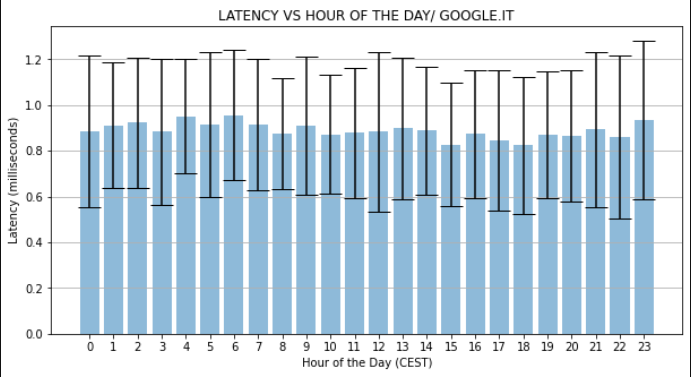
\includegraphics[scale=0.4]{latency_graph}
\caption{Latency Graph}
\label{fig:latency_graph}
\end{figure}

\begin{figure}[h!]
\centering
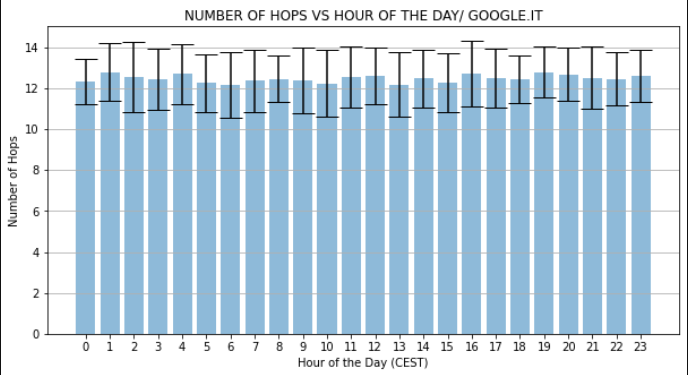
\includegraphics[scale=0.4]{hops_graph}
\caption{Hops Graph}
\label{fig:hops_graph}
\end{figure}


It doesn't appear that there is much confirmation for the suspected trend in either of the  two graphs, although it does seem, in Figure \ref{fig:latency_graph}, that the latency grows a little during the late evening (18 - 23). If latency is assumed to be proportional to server traffic, this may provide some support for the aforementioned idea that peak time happens during the evening hours.\\

For a more decisive answer, this experiment must be repeated for a much longer time interval, and perhaps leveraging many vantage points, stationed in different parts of the globe.

\section{Second Part}
In the second lab, the goal was to experiment with the DNS (Domain Name System), using an assortment of CLI tools designed to test the functioning and performance thereof.

\subsection{Methodology and experimental setup}
All of the tests were performed from the same local network at home.

\subsection{Part 1}

\subsubsection{Query the DNS to obtain the IP addresses of ercole.unipv.it and of another website in the domain it; are the answers authoritative? Why?}

Using the dig command, the IPs are: 193.204.34.13 and 142.250.180.163 (google.it). The answers aren't authoritative, as in both cases AUTHORITY flag returned is set to 0. This is because said answers aren't provided to us directly by the nameserver of the owner of the domain, but rather mediated through our local resolver.

\subsubsection{Query the DNS to obtain the name(s) of the mail servers associated with the
domain universitadipavia.it and berkeley.edu. How many servers
provide this service? Is there anything specific associated with the RRs?}

Using the dig command with the -t MX option (for MX RRs), it can be shown that there were 7 mail-servers associated to Pavia and 5 associated to Berkley. From their names one could tell that they're all actually Google servers; and this makes sense, since the managment of email in these organizations (at least in the case of Pavia) has long been outsourced to Google.


\subsubsection{Query the DNS to obtain the IP address of a Web server in Asia; is the answer
authoritative? Why? How many RRs did you obtain? What is their type? Does the
domain sign any RR type using DNSSEC?}

Querying the official website of the Japanese Government for RRs of type A, with the +dnssec option enabled in dig:\\

dig www.japan.go.jp @1.1.1.1 +dnssec\\

... yields a result that contains 4 type A RRs, in addition to an RRSIG record, and an "ad" (Authentic Data) flag in the flags section, which shows that dig believes the server to be using DNSSEC. \\

However, the AUTHORITY flag set to 0 shows that the answer isn't authoritative. This is again because it wasn't provided to us directly by the owner of the domain, but rather by Cloudflare's public name server.\\


As a sidenote, querying the one of the website's official name servers, does return an answer with an AUTHORITY that is not equal to 0.\\



1) dig -t NS japan.go.jp +short\\

\# results\\
ns-683.awsdns-21.net.\\
ns-360.awsdns-45.com.\\
ns-1588.awsdns-06.co.uk.\\
ns-1100.awsdns-09.org.\\


2) dig -t A ns-1100.awsdns-09.org. +short\\

\# results\\
205.251.196.76\\


3) dig japan.go.jp  @205.251.196.76\\

\# results\\
\# ... AUTHORITY : 4 ...


\subsubsection{Query the DNS to obtain the IP addresses of the authoritative Name Servers of a company outside Europe; how many queries did you execute? What type(s) of
queries? How many Name Servers are associated with the company? Do they
belong to the same domain? Can you identify the primary Name Server? Why?
Who registered the domain? When will it expire?}

A query was performed on the domain duolingo.com, like so:

dig duolingo.com -t NS 

These are the results of the query:\\

\begin{table}[h!]
\centering
\begin{tabular}{|l|l|l|l|l|}
\hline
duolingo.com. & 172800 & IN & NS & ns-1020.awsdns-63.net.   \\ \hline
duolingo.com. & 172800 & IN & NS & ns-1117.awsdns-11.org.   \\ \hline
duolingo.com. & 172800 & IN & NS & ns-1904.awsdns-46.co.uk. \\ \hline
duolingo.com. & 172800 & IN & NS & ns-247.awsdns-30.com.    \\ \hline
\end{tabular}
\label{fig:table3}
\end{table}

From the names of the nameservers you can tell that the are owned by Amazon AWS (Amazon Web Services), and that each of them is registered under a different TLD (Top Level Domain). \\

To obtain the IPs, it was necessary to perform a query for type A RRs on each single name in Table \ref{fig:table3}, so, in total, the queries executed were: 1 type NS and 4 type A queries.\\ The following are the IPs associated to each of the names:

\begin{table}[h!]
\centering
\begin{tabular}{|l|l|}
\hline
ns-1020.awsdns-63.net.   & 205.251.195.252 \\ \hline
ns-1117.awsdns-11.org.   & 205.251.196.93  \\ \hline
ns-1904.awsdns-46.co.uk. & 205.251.199.112 \\ \hline
ns-247.awsdns-30.com.    & 205.251.192.247 \\ \hline
\end{tabular}
\end{table}

Running the whois utility on awsdns-30.com, which was assumed to be the primary name sever: just because the associated webiste (duolingo.com) is registered under the same TLD, the Expiry Date was found to be: 2024-10-21T21:02:35Z.


\subsubsection{Query one of the Name Servers identified in the previous experiment to obtain the IP address of the Name Servers of the domains unipv.it and samsung.com.
How many IP addresses did you get?}

Zero, the queries returned a status REFUSED flag, and no answer. This is probably due to the fact that the name servers that were queried were not public, and hence wouldn't respond to a recursive query request, coming from without their domain, that involved iteratively querying external servers in the DNS hierarchy.\\

On the other hand, they did respond when queried about the domain duolingo.com, which they were supposed to know already.


\subsection{Part 2}


\subsubsection{Measure the performance of a Name Server when processing multiple queries. 
Did you notice any variability? Any expected/unexpected behavior?}


The tool used for this task was dnsperf, which happens not to be available on Aptitutde (Ubuntu's main package manager) as of writing this report, so it had to be built from source, following the steps on the tool's repository [\ref{article2}]

Cloudflare's public name server's performance was measured, with the five following queries repeated 1000 times each:

\begin{table}[h!]
\centering
\begin{tabular}{|l|l|}
\hline
www.usa.gov & A     \\ \hline
www.usa.gov & NS    \\ \hline
www.usa.gov & MX    \\ \hline
www.usa.gov & HTTPS \\ \hline
www.usa.gov & RRSIG \\ \hline
\end{tabular}
\end{table}

Among the 5000 total queries that were executed,  4863 returned with a NOERROR code, and 137 with a "T", which is dnsperf's way of saying that the query timed out.

The verbose option was turned on, to obtain the latency and response status of each single request. That data was then processed with Python, to obtain these average results for the latency in milliseconds. (average on the query type).

\begin{table}[h!]
\centering
\begin{tabular}{|l|l|}
\hline
A     & 0.056626 \\ \hline
HTTPS & 0.056006 \\ \hline
MX    & 0.056162 \\ \hline
NS    & 0.056179 \\ \hline
RRSIG & 0.056231 \\ \hline
\end{tabular}
\end{table}


From the table it seems that these times are all very similar, albeit the number of queries needed to establish that for sure, is many orders of magnitude greater than the total number of queries that were run in this example.


\subsubsection{Measure the performance of different Name Servers when processing the same
set of queries. Did the response time vary with the Name Server? Does it depend
on the type of query or on the geographic location of the Name Server?}

The tool dnseval was used for this task, querying the following nameservers: 

\begin{table}[h!]
\centering
\begin{tabular}{|l|l|}
\hline
Cloudflare & 1.1.1.1        \\ \hline
Google     & 8.8.8.8        \\ \hline
Cisco      & 208.67.222.222 \\ \hline
Quad9      & 9.9.9.9        \\ \hline
\end{tabular}
\label{fig:table4}
\end{table}

For each of the aforementioned nameservers, and for each of the following five RR types,
the domain google.com was queried 50 times (-c option of the dnseval command). 


\begin{table}[h!]
\centering
\begin{tabular}{|l|l|}
\hline
A    \\ \hline
NS     \\ \hline
MX \\ \hline
HTTPS              \\ \hline
RRSIG              \\ \hline
\end{tabular}
\label{fig:table4}
\end{table}


The first thing to be noticed, was that -t HTTPS returned an error, indicating that it wasn't considered a valid RR type by dnseval, perhaps owing to its novelty with respect to the more traditional RR types.\\

Other than that, in terms of speed (average latency in ms), Cisco's nameserver turned out to be the slowest. This didn't seem to depend on the geographic location of the name servers themselves, as all of the aforementioned servers are located in the US, with the exception of Cloudflare's, located in Australia, according to Keycdn [\ref{article3}] 

Another thing worth noting, is that only Cisco's name server didn't respond at all when queried for the RRSIG records associated to the domain name google.com.

It could be concluded that the difference in performance in this experiment depended on the query type, as well as the geographic location of eventual CDNs (Content Delivery Networks) or some other factor, but probably not on the geographic location of the name servers themselves, as they were all located very far away from the vantage point, the latter being in Italy.


\subsubsection{Check the path followed by your queries using different Name Servers; did you
notice any expected/unexpected behavior?}

The command dnstraceroute was employed for this task. As expected, the routes started out pretty much identical, then they began diverging (at approximately hop 7). 

It took 12 hops to reach Google's and Quad9's name servers, 11 hops to reach Cloudflare's name server and just 10 hops to reach Cisco's name server, despite it scoring the largest latency on the previous experiment.


% idk, latex just needs this here for bibliography linking to work properly:
\clearpage

\section{Conclusions}

You can find the code employed in these experiments on Github [\ref{article4}] 

\section{References}

\begin{enumerate}

\item \label{article1}  \url{https://www.highspeedinternet.com/resources/why-does-my-internet-slow-down-at-night} 
\item \label{article2}  \url{https://github.com/DNS-OARC/dnsperf} 
\item \label{article3}  \url{https://tools.keycdn.com/geo?host=1.1.1.1+} 
\item \label{article4}  \url{https://github.com/aiman-al-masoud/edi_reports} 

\end{enumerate}





\end{document}